\chapter{Introduction}
This is a template for writing a thesis according to the Technion specifications. 
Please, however, check with the graduate school website to see if any specifications have changed. 
This template was written by Boaz Shuval (January 2019). 

\section{Instructions}

This template is provided as is. Please check with the Technion graduate school website to see if the guidelines have changed, as they often do. For
the latest directions from the graduate school, see: 
\url{https://graduate.technion.ac.il/graduation/thesis-editing/}
(This is the website address circa January 2019). 

All files use UTF-8 encoding. Make sure your LaTeX system supports this encoding. 

\subsection{Preparing the Thesis}

\begin{enumerate}
\item The main.tex file is the main file to be compiled. Place it (with the other thesis files) in the same directory as the \verb".cls" and \verb".sty"
    files provided.                                                                                                                                          
    \item  The main class is \verb"technionThesis.cls."
   It has the the following options:  
   \begin{itemize}
       \item  hyperref       ---  Add hyperlinks
       \item  publist        ---  Add a list of publications in the front pages (update list in thesissetup.sty)
       \item  addack         ---  Add an acknowledgments page (only for final version!)
       \item  advisement     ---  Use "advisement" instead of "supervision" in front pages (a pet peeve of mine)
       \item  spacepar       ---  Add a blank line between paragraphs
       \item  firstparindent ---  Indent the first paragraph of a chapter/section
       \item  libertine      ---  Use a different selection of fonts, based on libertine, for the English part of the thesis. (See note 4)
    \end{itemize}
\item In the file \verb"technionThesisSetup.sty" you must input your details in the various commands. It is pretty self explanatory. 
\item The class loads a number of packages that the class author (Boaz Shuval) uses regularly. It also sets up theorem-style environments.
   If you know what you're doing, feel free to change things as you see fit. Otherwise, leave this alone. 
   \begin{enumerate}
       \item Environments are defined using amsthm. The following environments are available:
           \begin{itemize}
               \item Theorem-style: theorem, lemma, corollary, proposition, conjecture
      (Heading in bold, text in italics)
      These all share consecutive numbering, in the format (chapter.number)
  \item Definition-style: definition, example, assumption, condition 
      (Heading in bold, text upright)
      These are numbered (chapter.number) with their own numbering. Assumption and condition have alphanumeric numbering (A,B,C, etc.)
  \item Remark-style: remark, question, discussion
      (Heading in italics, text upright)
      These are numbered (chapter.number) with their own numbering. Discussion is unnumbered. 
  \item Proof environments: proof, IEEEproof. Both have a black square at the proof end. 
    \end{itemize}
\item  Packages loaded (partial listing):
    \begin{itemize}
        \item mathtools (which loads amsmath)
        \item amsthm, amssymb
        \item IEEEtrantools (loads IEEEeqnarray, and also sets the bibliography style)
        \item graphicx 
        \item tikz (including various useful tikz libraries) 
        \item cleveref (for referring to sections, etc, using \verb"\Cref", automagically adding the header)
        \item stackrel
        \item accents  (for adding symbols above symbols)
        \item xspace (for adding a smart space after a macro command)
        \item tabto  (add a tabstop for lining things up)
        \item algorithm2e (ruled, vlined)
        \item url
        \item polyglossia (for Hebrew support)
        \item longtable (for a table that runs over more than one page; useful for the abstract)
        \item booktabs, multirow (for nicer tables)
    \end{itemize}
    \end{enumerate}
\item Place all of your own commands in the file \verb"Example/technionThesisMacros.sty". That is, various \verb"\newcommand" and \verb"\DeclareMathOperator" are defined here. I've defined a few
   useful ones for you to get started. 
\item There are now \verb".tex" files for you to edit: 
    \begin{itemize}
        \item \verb"abstract.tex"         for your abstract in English (200-500 words)
        \item \verb"habstract.tex"        for your abstract in Hebrew (500-2000 words)
        \item \verb"acknowledgments.tex"  for your acknowledgments in English
        \item \verb"hacknowledgments.tex" for your acknowledgments in Hebrew
        \item \verb"introduction.tex"     for your introduction chapter
        \item \verb"chapfirst.tex"        for your first chapter 
        \item \verb"chapsecond.tex"       for your second chapter (add additional chapters as you see fit)
        \item \verb"discussion.tex"       for your discussion/conclusions chapter
        \item \verb"appendix.tex"         for your appendix (appendices must appear in their own chapters, and not as part of the main text). 
   \end{itemize}
   \end{enumerate}

   \subsection{Compilation}
Compile using xelatex. If you are using latexmk, you may include in the compilation directory a file called \verb".latexmkrc"
with the following line: 

\verb"$pdflatex = 'xelatex --shell-escape %O %S';"

This tells latexmk to use xelatex for compilation, so you need not worry
about this.
You may also compile this on overleaf (again, use xelatex). 

The Hebrew portion of the thesis is based on the polyglossia package. It uses the David CLM font for Hebrew. Thus, you must install the culmus fonts
for this to work on your installation. 

\subsection{ Be a pal}
Please share this template with your friends and colleagues. 
If you enjoyed using it, consider sending me a note to let me know. 
If you find a bug, or have asuggestion for improvement, I'd love to know about it.

\section{Files in this Template}

\begin{itemize}
    \item  \verb"technionThesis.cls"     ---  The class file
    \item  \verb"technionThesisSetup.sty"        ---  Setup data fields
    \item  \verb"README.md"                
    \item  Inside the Example directory:
        \begin{itemize}
    \item  \verb"abbrev.tex"               
    \item  \verb"abstract.tex"             
    \item  \verb"acknowledgments.tex"
    \item  \verb"appendix.tex"
    \item  \verb"chapfirst.tex"
    \item  \verb"chapsecond.tex"
    \item  \verb"discussion.tex"
    \item  \verb"habstract.tex"          ---  Hebrew abstract
    \item  \verb"hacknowledgments.tex"   ---  Hebrew acknowledgments
    \item  \verb"introduction.tex"
    \item  \verb"main.tex"               ---  Main thesis file
    \item  \verb"mybib.bib"
    \item  \verb"technionThesisMacros.sty"           ---  Define your macros here
\end{itemize}
\end{itemize}

\section{License}
This template is licensed under Creative Commons CC BY 4.0. 

\section{Notes}
\begin{enumerate}
    \item This template was tested on a mac running macOS 10.13, with TEXLIVE2017. It was also tested on overleaf in January 2019, which also runs TEXLIVE2017. 
    \item There is a bug when using TEXLIVE2018, which manifests itself in the figure/table numbering. If you encounter this bug, use the memoir package from
          TEXLIVE2017, instead. 
    \item The template uses the Memoir package internally. The chapter heading design is a modified version of a design by Vincent Zoonekynd 
        (it is modified from the BlueBox style in \url{https://ctan.org/pkg/memoirchapterstyles}).  
       \item If using the libertine option, make sure to use the latest version of newtxmath, available from \url{https://ctan.org/pkg/newtx}
   (download the file \verb"newtxmath.sty" to the home directory)
   \end{enumerate}


   \section{ Version History}
31 January 2019:    Version 1.0




\section{A Section} 
The remainder of this file is a boilerplate example
Equations are also fine: 
\[ 
    f(x) = x+2,
\] 
as are numbered equations:
\begin{equation}\label{eq:numbered int}
    g(y) = y.
\end{equation}
Of course, one may refer to a numbered equation such as~\eqref{eq:numbered int}. 

\section{Second section}
In this section we have a figure. 

\begin{figure}[t]
    \begin{center}
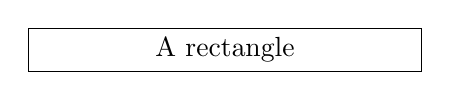
\begin{tikzpicture}
    \node[draw, minimum width = 5cm] {A rectangle};
\end{tikzpicture}
\end{center}
\caption[Short caption]{A very long caption for this figure. It is deliberately very long to illustrate the usefulness of the short caption for the table of figures. }
\label{fig:rectangle}
\end{figure}
\lipsum[10-13]















